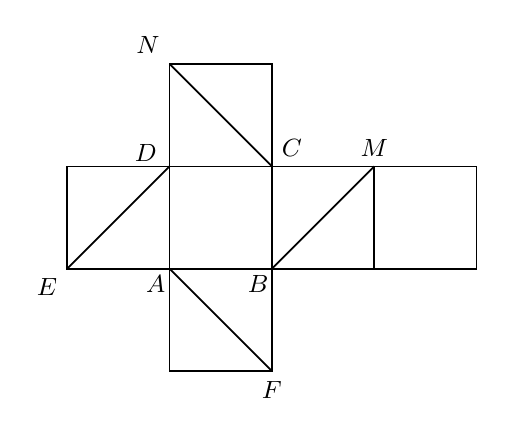
\begin{tikzpicture}[line width=0.6pt, font=\small]
  % unit 1.3; coordinates written literally (no implicit-multiplication macros)
  % center square ABCD: (0,0),(1.3,0),(1.3,1.3),(0,1.3)
  \draw (0,0) rectangle (1.3,1.3);
  % top square
  \draw (0,1.3) rectangle (1.3,2.6);
  % left square
  \draw (-1.3,0) rectangle (0,1.3);
  % bottom square
  \draw (0,-1.3) rectangle (1.3,0);
  % right squares
  \draw (1.3,0) rectangle (2.6,1.3);
  \draw (2.6,0) rectangle (3.9,1.3);
  % four diagonals
  \draw (0,2.6) -- (1.3,1.3);
  \draw (-1.3,0) -- (0,1.3);
  \draw (1.3,0) -- (2.6,1.3);
  \draw (0,0) -- (1.3,-1.3);
  % labels
  \node[above left] at (0,2.6) {$N$};
  \node[left,xshift=-1pt,yshift=5pt] at (0,1.3) {$D$};
  \node[above right] at (1.3,1.3) {$C$};
  \node[above] at (2.6,1.3) {$M$};
  \node[below left] at (-1.3,0) {$E$};
  \node[below,xshift=-5pt,yshift=1pt] at (0,0) {$A$};
  \node[below,xshift=-5pt,yshift=1pt] at (1.3,0) {$B$};
  \node[below] at (1.3,-1.3) {$F$};
\end{tikzpicture}
